% 2025-02-13
\documentclass{article}
\usepackage{latexsym}
\usepackage{amsmath}
\usepackage[a4paper]{geometry}
\usepackage{fullpage}
\usepackage{hyperref}
\usepackage{booktabs}
\usepackage{graphicx}
\usepackage{tikz}
\usepackage{xcolor}
\usepackage[export]{adjustbox}
\usepackage{comment}
\usepackage{subcaption}
\usepackage[style=iso]{datetime2}
\usepackage{cleveref}
%\usetikzlibrary{calc}
\usetikzlibrary{arrows,positioning} 
\tikzset{
    %Define style for course boxes
    courseboxv/.style={
           rectangle,
           draw=blue!50!black, very thick,
           fill=blue!10,
           minimum height=8cm,
           minimum width=4cm,
           text width=3.9cm,
           text centered,
           font=\bfseries\sffamily},
    courseboxh/.style={
           courseboxv,
           minimum height=4cm,
           minimum width=8cm,
           text width=7.9cm},
    courseboxhh/.style={
           courseboxh,
           minimum height=4cm,
           minimum width=16cm,
           text width=15.9cm}
}
\def\frameseparation{1.5cm}
\def\scalingfactor{.8}

\newcommand{\secref}[1]{Section~\ref{sec:#1}}
\newcommand{\secreff}[2]{Sections \ref{sec:#1} and \ref{sec:#2}}
\newcommand{\eqnref}[1]{Equation~\eqref{eq:#1}}
\newcommand{\eqnreff}[2]{Equations \eqref{eq:#1} and \eqref{eq:#2}}
\newcommand{\eqnrefff}[3]{Equations \eqref{eq:#1}, \eqref{eq:#2} and \eqref{eq:#3}}
\newcommand{\figref}[1]{Figure \ref{fig:#1}} 
\newcommand{\figreff}[2]{Figures \ref{fig:#1} and \ref{fig:#2}}
\newcommand{\figrefff}[3]{Figures \ref{fig:#1}, \ref{fig:#2} and \ref{fig:#3}}
\newcommand{\tabref}[1]{Table~\ref{tab:#1}}
\newcommand{\tabreff}[2]{Tables~\ref{tab:#1} and \ref{tab:#2}}
\newcommand{\tabrefff}[3]{Tables~\ref{tab:#1}, \ref{tab:#2} and \ref{tab:#3}}

\def\year{2024--2025}
\title{EITA65 Design of Systems for Digital Transformation\\\year}
%\title{EITA65 Digitalisering -- realisering och systemdesign med användarperspektiv\\\year}
\author{\huge Configuring a Private Network\\Drone Project -- Part 4}
%\\Version \DTMnow}
%\date{}

\begin{document}
\newgeometry{left=2.5cm,right=2.5cm,bottom=1.5cm}% for placing course schematic lower on first page
\clearpage\maketitle
\thispagestyle{empty}% to remove page numbering on first page

\begin{itemize}
\item \includegraphics[width=3mm]{person.png}\includegraphics[width=3mm]{person.png}\includegraphics[width=3mm]{person.png}\includegraphics[width=3mm]{person.png} In this project, you will work together in groups  of 3 or 4 -- the same groups you will do your project with in study period 4. See Canvas under \emph{Persons/Project Groups} for a list of the groups.
\item You will not get detailed step-by-step instructions. Figuring out how to reach the goal is part of the project (being a collaborative doer).
\item The results of this project part will be used in the next, so document your work.
\end{itemize}

\vspace{.1cm}
\begin{center}
\begin{tabular}{l}
\toprule[1.5pt]
\parbox{0.8\linewidth}{
\vspace{.2cm}{\Large Learning goals:}
\begin{itemize}
    \item Configuring a local area network (LAN) by yourself
    \item Getting a communication-centered system view by studying how different system sub-components communicate via HTTP
    \item Practicing active collaboration with your group members.
\end{itemize}}\\
\bottomrule[1.5pt]
\end{tabular}
\end{center}
\vfill
% \begin{center}
% \includegraphics[width=120mm]{rpi4_no_bg.png}
% \end{center}
%\vspace{2cm}
\begin{center}
\includegraphics[width=70mm]{router.png}
\end{center}

\begin{comment}
\begin{center}
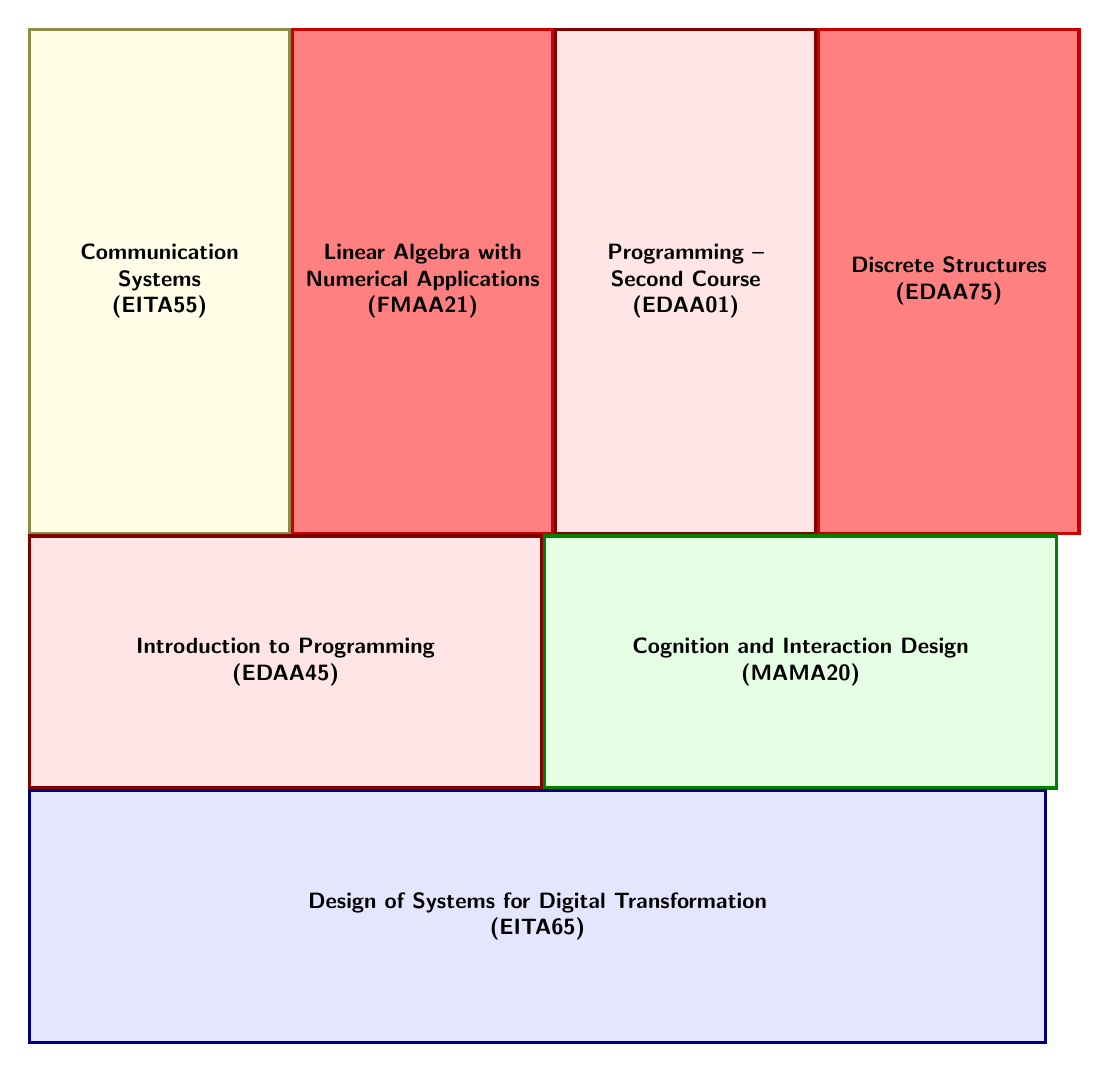
\begin{tikzpicture}[>=latex, node distance=0cm,scale=\scalingfactor,every node/.style={scale=\scalingfactor}]
\node[courseboxv, draw=yellow!50!black, fill=yellow!10] (EITA55) {Communication Systems\\(EITA55)};
\node[courseboxv, draw=red!80!black, fill=red!50, anchor=west] (FMAA21) at (EITA55.east){Linear Algebra with Numerical Applications\\(FMAA21)};
\node[courseboxv, draw=red!50!black, fill=red!10, anchor=west] (EDAA01) at (FMAA21.east){Programming -- Second Course\\(EDAA01)};
\node[courseboxv, draw=red!80!black, fill=red!50, anchor=west] (EDAA75) at (EDAA01.east){Discrete Structures\\(EDAA75)};
%\node[courseboxh, preaction={clip, postaction={fill=red!10, draw=red!50!black, line width=2mm}}, anchor=north west] (EDAA45) at (EITA55.south west){Introduction to Programming\\(EDAA45)};
\node[courseboxh, draw=red!50!black, fill=red!10, anchor=north west] (EDAA45) at (EITA55.south west){Introduction to Programming\\(EDAA45)};
%\node[courseboxh, draw=green!50!black, fill=green!10, anchor=west] (MAMA20) at (EDAA45.east){Cognition and Interaction Design\\(MAMA20)};
\node[courseboxh, draw=green!50!black, fill=green!10, right=of EDAA45] (MAMA20) {Cognition and Interaction Design\\(MAMA20)};
\node[courseboxhh, anchor=north west] (EITA65) at (EDAA45.south west){Design of Systems for Digital Transformation\\(EITA65)};
%\node[anchor=south east, inner sep=2pt, font=\bfseries\sffamily\scriptsize] at (EDA625.south east) {Helsingborg};
%\path[->,draw=black,dotted,thick] (EIT060.east) -- (EITF05.west);
%\path[->,draw=black,dotted,thick] (EIT060.south) -- (EITN50.north);
%\path[->,draw=black,dotted,thick] (EITF05.south) -- (EITN41.north);
%\draw[draw=blue!50!black, very thick] ($(EIT060.north west)+(-\frameseparation,\frameseparation)$) rectangle ($(EDA625.south east)+(\frameseparation,-\frameseparation)$);
\end{tikzpicture}
\end{center}
\end{comment}

\restoregeometry
\newpage


\section{Introduction}
In this part, you will need to recall some things you learned in the recent lecture about computer networks. You will configure a local area network that is shared with your group members. There is something you need to know before you come to the lab.
\begin{itemize}
    \item Each group (with 3 or 4 members) will get a switch, and each member in the group will get an Ethernet cable. Together, you will use the switch and the cables to build a wired private network connecting the Raspberry Pis of all group members in this lab.
    \item Each group needs to bring at least two Raspberry Pis to the lab, each group may occupy two lab computers during the lab session to finish their task.
    \item If you wish you can replace the Raspberry Pi with your own laptop, but in the lab, you need to build a network for all devices that are involved in the system. However, be aware that your supervisors might not be experts in how to configure your particular system and may perhaps only be able to provide limited help.
    \item You will not be given step-by-step introductions on how to build a network, so if you don't remember anything about computer communication or networks, it is a good idea to brush up your skills by consulting a text book or searching the Internet.
\end{itemize}

\section{Building Your Network}
\subsection{Connecting the Hardware}
Before starting, turn on the switch and connect the Raspberry Pis to the switch. You will build the private network using the Ethernet interfaces, but it is a good idea to also have the Raspberry Pis connected to WiFi, so that you have access to the Internet for package updating and upgrading.
\subsection{Configuring the IP addresses}
As you learned in the computer network lecture, an IP address consists of two parts, \emph{network id} and \emph{host id}. Two hosts in the same local network should have identical network id and different host ids. An IPv4 (Internet Protocol version 4) address consists of 32 bits, often written as four eight-bit numbers. Depending on how large the local network is (number of nodes), the number of bits reserved for the network id (and consequently also for the host id) can vary. By specifying a \emph{net mask} you can control which bits of the IP address is a part of the network id and which belong to the host id. When your Raspberry Pi, or another computer on the local network, sends a data package over the network, it will use the net mask to determine whether the destination computer is on the same local network or not. In the first case package will be sent directly to the destination computer. In the latter case the package will instead be sent to a \emph{gateway} which will relay the message to another network. Your computer also uses the net mask and the IP addresses assigned to the network interfaces to decide which interface to use to send the package -- the Ethernet port or the WiFi connection.\\

\noindent{\bf Question 1: }\parbox[t]{14cm}{\textcolor{red}{Before you start configuring the IP on your Raspberry Pis, write down the network id you intend to use for your network, as well as the net mask and the IP addresses you will assign to the various Raspberry Pis.}}\\

\noindent{\bf Question 2: }\parbox[t]{14cm}{\textcolor{red}{Write down the name of network interface that you will assign the IP address to.}}\\

\noindent{Note: }\parbox[t]{14cm}{We do realize that these are not actually questions, but that it is essential to your work.}\\

\noindent Now you can assign IP addresses to the Raspberry Pis. There are various ways to assign IP addresses to an interface.
You can use the command \verb!ip addr add <address/netmask> dev <interface>! to temporarily configure the network or you can permanently put the address in the network settings of your Raspberry Pis using the GUI (network icon -- advanced options -- edit connections). The latter is probably the best option. Make sure that you have the network mask configured correctly and that you assign the IP address \emph{manually} (static IP) and not \emph{automatically} (dynamic IP).

\noindent Once you correctly assign the IP addresses, your Raspberry Pis should be able to communicate with each other. Verify using \verb!ping! that you have a working connection between the different Raspberry Pis in your network.

Another useful tool is the command \verb!ip addr! which lists the properties, including ip addresses, of all your interfaces. It can help you determine the names of your interfaces and which IP number, if any, is associated with them.

\section{Deploying the Drone System}
Once you have your network configured successfully, deploy the drone system on the Raspberry Pis. Clone the {\color{blue}\href{https://github.com/rogerhenriksson/InfoCom-Drone-4-Private_Network}{GitHub Repository}} (\href{https://github.com/rogerhenriksson/InfoCom-Drone-4-Private_Network}{https://github.com/rogerhenriksson/InfoCom-Drone-4-Private\_Network}) to both Raspberry Pis in your network. In this lab we will use one Raspberry Pi to run the servers and another to run the drone simulation (you will thus need a total of two Raspberry Pis for this task). The system architecture is shown in \Cref{fig:sys}.
\begin{figure}
    \centering
    \includegraphics[width=\linewidth]{architecture.png}
    \caption{System architecture}
    \label{fig:sys}
\end{figure}

The system setup here is different from that in the previous assignments. The drone part is now moved to a separate Raspberry Pi (Pi One in \Cref{fig:sys}). Therefore, in order for the route planner to be able to send address information to the drone, we need to have the Raspberry Pis communicate via the network through IP addresses. Therefore, the Drone Pi also needs to run a flask server (\verb!drone.py!) in order to listen to requests from the route planner.

\noindent Once the Drone Pi receives coordinates, it starts the simulation and updates its location to the Redis database, which is hosted on the Server Pi. Thus, both Pis need to know each other's IP addresses in order to communicate. Open the code files on both Raspberry Pis, replace the {\bf REDIS\_SERVER}\footnote{Also check the connection to the Redis database in \texttt{routeplanner.py}.} and {\bf DRONE\_IP} with the correct addresses on Server Pi, and replace {\bf WEBSERVER\_IP} on the Drone Pi. You will also need to update \texttt{simulator.py}. Then run the system following the instructions in \verb!README.md!. If everything is configured correctly, you should be able to input addresses in your browser and see the drone moving on the map, as in LP2. When you have finished all the tasks in this part, show the TA your working system.
% {\bf Hint 1: }\parbox[t]{14cm}{Check for updates to this document. Instructions may have been clarified in a more recent version. You can find the version number of the document on the very first page. The version number is the compile-date of the document in ISO-format~\cite{iso-date-time}.}\\
% {\bf Hint 2: }\parbox[t]{14cm}{To avoid rewriting many commands, you can use the keys \texttt{arrow up} and \texttt{arrow down} to go back and forth between the commands that you just wrote.}\\
% {\bf Hint 3: }\parbox[t]{14cm}{To paste commands into the terminal you can use \texttt{Ctrl + Shift + V}}\\
% {\bf Hint 4: }\parbox[t]{14cm}{tab in instructions}\\
% {\bf Hint 5: }\parbox[t]{14cm}{To avoid rewriting many commands, it can be a good idea to write all steps in a batch-file or shell script. Then you can also reuse the batch file for the second project.}
%\vspace{1cm}
\begin{center}
\huge Good luck!
\end{center}

% \begin{thebibliography}{10}
% \bibliographystyle{plain}

% \bibitem{OSM} OpenStreetMap, \url{https://www.openstreetmap.org/#map=14/55.7059/13.2005}, last accessed on 2022-01-20.

% \bibitem{deco} Python decorator, \url{https://python-3-patterns-idioms-test.readthedocs.io/en/latest/PythonDecorators.html}, last accessed on 2022-01-20.


% \end{thebibliography}

\end{document}
